An AVL tree \cite{avl:original} is a self-balancing binary search tree, where the absolute value of the height difference between two child subtrees is no more than one.
This may also be described by the \textit{balancing factor}.

\begin{definition}[Tree height]
  \label{def:height}
  The height of a node in a tree is the maximal number of edges from that node to a leaf.
\end{definition}

\begin{definition}[Balancing factor]
  \label{def:balancing_factor}
  The balancing factor of any node is defined to be the height difference of its two child subtrees.
\end{definition}

In Lean, the definitions \lstinline{height} and \lstinline{balanced} are done per Definitions \ref{def:height} and \ref{def:balancing_factor}.

\begin{lstlisting}
def height : btree α → nat
| btree.empty := 0
| (btree.node l k a r) :=
  1 + (max (height l) (height r))

def balanced : btree α → bool
| btree.empty := tt
| (btree.node l k a r) :=
  if height l ≥ height r 
    then height l ≤ height r + 1
    else height r ≤ height l + 1
\end{lstlisting}

The process of looking up a node or searching for a key is the same as in BSTs. During insertion and deletion, however, a tree may become unbalanced, after which rotation algorithms are used to re-balance the tree. A tree can either be left-heavy or right-heavy. Left-heaviness can be fixed with a simple right rotation; right-heaviness with a simple left rotation. If the subtrees of the children are also unbalanced, compound rotations are used to re-balance, which consist of a right rotation followed by a left rotation or vice versa.

A tree \lstinline{t} being left-heavy means that if the right subtree has a height of $n$, the height of the left subtree is $n+2$; similarly, a right-heavy tree has a left subtree of height $n$ and a right subtree of height $n+2$. The definitions presented further closely follow \cite{textbook:discrete_computer}. The definition for \lstinline{right_heavy} is mirrored.

\begin{lstlisting}
def left_heavy : btree α → bool
| btree.empty := ff
| (btree.node btree.empty k a r) := ff
| (btree.node (btree.node ll lk la lr) k a r) :=
  (height ll ≥ height lr) ∧ (height ll ≤ height lr + 1) ∧
  (height lr ≥ height r) ∧ (height r + 1 = height ll)

def simple_right : btree α → btree α
| btree.empty := btree.empty
| (btree.node (btree.node ll lk la lr) k a r) := 
    btree.node ll lk la (btree.node lr k a r)
| (btree.node l k a r) := btree.node l k a r
\end{lstlisting}

\begin{figure}[!ht]
  \begin{subfigure}{0.5\textwidth}
    \centering
    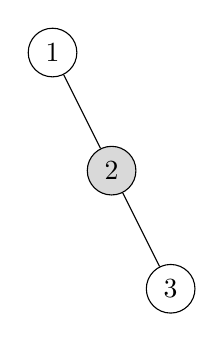
\begin{tikzpicture}
      \node[circle,draw](z){1}
        child[missing]{}
        child{
          node[circle,draw,fill=gray!30]{2} 
            child[missing] 
            child{
              node[circle,draw]{3}
              child[missing]
            }
          };
      \end{tikzpicture}
  \end{subfigure}%
  \begin{subfigure}{0.5\textwidth}
    \centering
    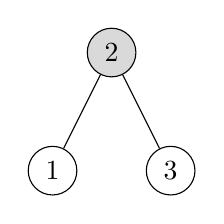
\begin{tikzpicture}
      \node[circle,draw,fill=gray!30](z){2}
        child{
          node[circle,draw]{1}
            child[missing]
            child[missing]
        }
        child{
          node[circle,draw]{3}
            child[missing]
            child[missing]
        };
    \end{tikzpicture}
  \end{subfigure}
  \label{fig:rotation}
  \caption{An example of a simple left rotation on a right-heavy tree.}
\end{figure}

In a simple right rotation, the pivot of the rotation is the left subtree, which is rotated. In a simple left rotation, the pivot of the rotation is the right subtree.

\begin{lstlisting}
def rotate_right : btree α → btree α
| btree.empty := btree.empty
| (btree.node l k a r) :=
  match l with
  | btree.empty := (btree.node l k a r)
  | (btree.node ll lk la lr) :=
    if height ll < height lr 
    then simple_right (btree.node (simple_left l) k a r)
    else simple_right (btree.node l k a r)
  end 
\end{lstlisting}

With simple rotations, only the height of the right (or left) child subtree matters. If the subtrees of the child are also too tall, i.e. too tall on the \enquote{inside}, a compound rotation needs to be applied. In the definition \lstinline{rotate_right}, the children of the left child are compared. If the left subtree of the child is smaller, a compound rotation is done as the tree is too heavy on the "inside". Otherwise, just a simple right rotation is done.

Deletion is more complicated, and depends on the placement of the node within the tree. If the left subtree is empty, then the node can be safely replaced by the right subtree.  If the left subtree has children, it can be of any height, so re-balancing has to be taken into account. In this case, the same philosophy can be followed as for deletion when the left subtree is empty, but traveling down the right subtree and looking for an empty right child. If a node \lstinline{n} is found with an empty right child, the key and data value of \lstinline{n} is returned, and \lstinline{n} is replaced by its left child subtree, with right rotations performed to restore balance. 

\begin{lstlisting}[escapeinside={*}{*}]
def shrink : btree α → option (nat × α × btree α)
| btree.empty := none
| (btree.node l k v r) := some *\$*
  match shrink r with
  | none := (k, v, l)
  | some (x, a, sh) :=
    if height l > height sh + 1
      then (x, a, rotate_right (btree.node l k v sh))
      else (x, a, btree.node l k v sh)
  end
\end{lstlisting}

Since shrinking an empty tree is impossible, \lstinline{shrink} returns an \lstinline{option}.

The next step is to define the steps to delete a node. This is done with the function \lstinline{del_node}. If the left subtree of the node to be deleted is not empty, then the left subtree is shrunken, and a new tree is formed with the resulting key from the shrink operation as the new node, the shrunken tree and the original right subtree. A rotation is done if the result is unbalanced. 

\begin{lstlisting}
def del_node : btree α → btree α
| btree.empty := btree.empty
| (btree.node l k v r) :=
  match shrink l with 
  | none := r
  | some (x, a, sh) :=
    if height r > height sh + 1 then rotate_left (node sh x a r)
    else node sh x a r
  end
\end{lstlisting}

Finally, the full \lstinline{delete} function is complete. 

\begin{lstlisting}
def delete (x : nat) : btree α → btree α
| btree.empty := btree.empty
| (btree.node l k a r) :=
  let dl := delete l in
  let dr := delete r in
  if x = k then del_node (btree.node l k a r)
  else if x < k then
    if height r > height dl + 1 then rotate_left (btree.node dl k a r)
    else btree.node dl k a r
  else if height l > height dr + 1 then rotate_right (btree.node l k a dr)
  else (btree.node l k a dr)
\end{lstlisting}

First, find the node to delete. If it is found, then the \lstinline{del_node} function is called on the entire subtree. During the search of the node to delete, the operation is called recursively, and rotations are applied if the tree becomes unbalanced. 